\documentclass[aspectratio=169,11pt]{beamer}
\usepackage[utf8]{inputenc}
\usepackage{graphicx}
\usepackage{amsmath,amssymb}

\usetheme{Madrid}
\usecolortheme{seahorse}
\setbeamertemplate{navigation symbols}{}
\setbeamertemplate{footline}{}
\setbeamersize{text margin left=7mm,text margin right=7mm}

\definecolor{ink}{HTML}{153242}
\definecolor{slate}{HTML}{465965}
\definecolor{accent}{HTML}{C85B34}
\setbeamercolor{normal text}{fg=ink,bg=white}
\setbeamercolor{structure}{fg=ink}
\graphicspath{{figures/}{./}}


\begin{document}
\begin{frame}[plain]
  \vspace*{0pt}
  {\color{ink}\fontsize{20.74}{24}\selectfont\bfseries
   Binned inference for the ETAS background\par}


  \vspace{1mm}
  \begin{center}
    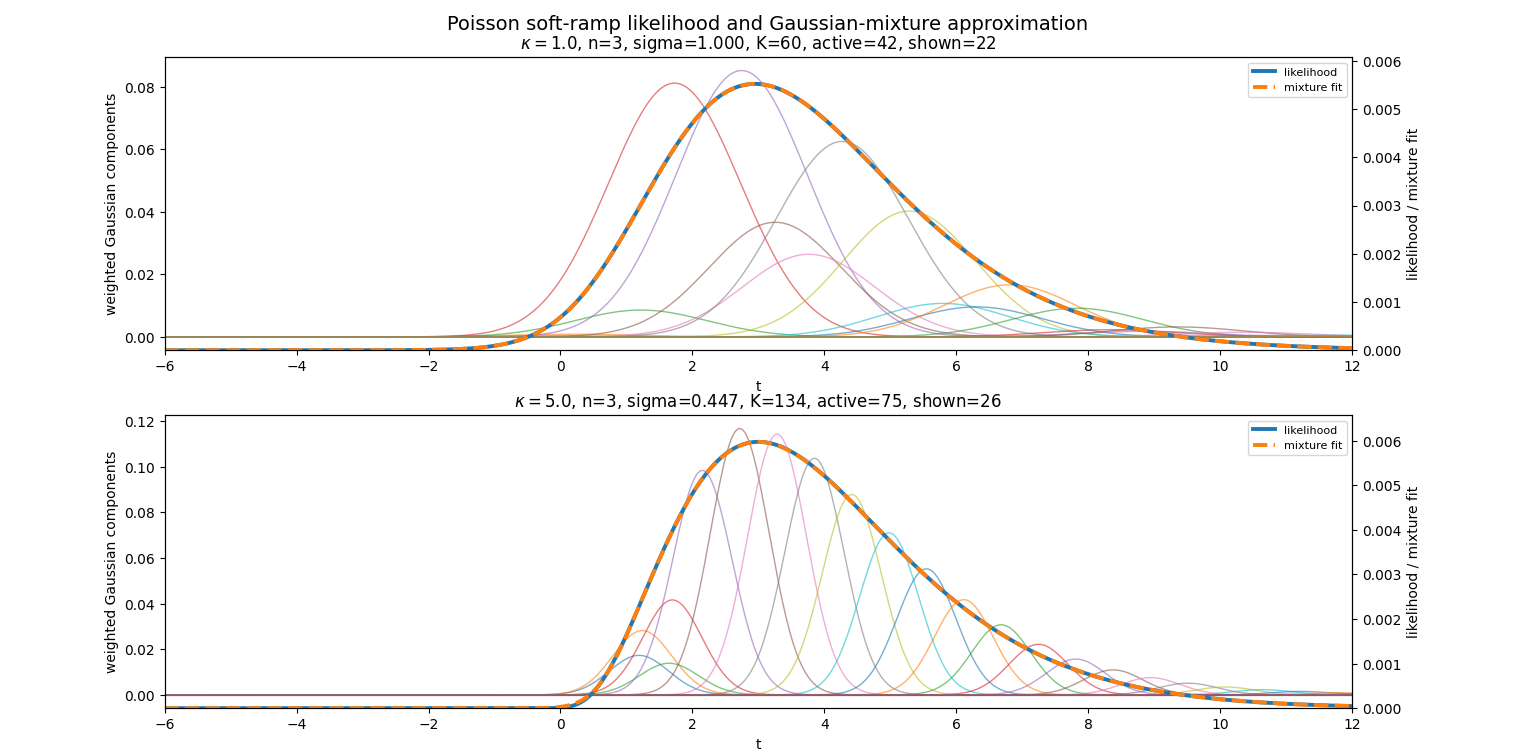
\includegraphics[
      width=0.99\textwidth,
      trim=0bp 259.92bp 0bp 24.48bp,
      clip
    ]{likelihood_mixture_k1_k5.png}
  \end{center}
  \vspace{-2mm}

  \begin{columns}[T,onlytextwidth]
    \begin{column}{0.31\textwidth}
      {\color{accent}\bfseries\fontsize{10}{12}\selectfont
       POINTWISE GP-ETAS\par}
      \vspace{1mm}
      {\fontsize{10.95}{13}\selectfont
       $\mathcal O((N_D+N_\Pi)^3)$\\
       \textcolor{slate}{Molkenthin et al.\ (2022)}\par}
    \end{column}

    \begin{column}{0.33\textwidth}
      {\color{accent}\bfseries\fontsize{10}{12}\selectfont
       BINNED LIKELIHOOD\par}
      \vspace{1mm}
      {\fontsize{10.95}{13}\selectfont
       $n_i^{\mathrm{bg}}\mid f_i
          \sim\mathrm{Poisson}(\Lambda_i)$\\
       $\Lambda_i=L(f_i)$;
       \textcolor{slate}{softplus / exp}\par}
    \end{column}

    \begin{column}{0.31\textwidth}
      {\color{accent}\bfseries\fontsize{10}{12}\selectfont
       MIXTURE AUGMENTATION\par}
      \vspace{1mm}
      {\fontsize{10.95}{13}\selectfont
       $\ell_n(f)\approx\sum_r w_r\mathcal N_r(f)$\\
       $Q_{\mathrm{post}}=Q+D^{-1}$\par}
    \end{column}
  \end{columns}

  \vspace{3mm}
  {\fontsize{9}{11}\selectfont
   Cristina O. Ch\'avez Chong\quad
   {\color{slate}Universität Potsdam}\hfill
   \href{mailto:cristina.chavez@uni-potsdam.de}
        {\texttt{cristina.chavez@uni-potsdam.de}}\par}
\end{frame}
\end{document}